\documentclass[a4paper, 12pt]{article}%тип документа

%отступы
\usepackage[left=2cm,right=2cm,top=2cm,bottom=3cm,bindingoffset=0cm]{geometry}
\setlength{\parindent}{5ex}

%Русский язык
\usepackage[T2A]{fontenc} %кодировка
\usepackage[utf8]{inputenc} %кодировка исходного кода
\usepackage[english,russian]{babel} %локализация и переносы

%Вставка картинок
\usepackage{graphicx}
\graphicspath{{pictures/}}
\DeclareGraphicsExtensions{.pdf,.png,.jpg}

%Графики
\usepackage{pgfplots}
\pgfplotsset{compat=1.9}

%Математика
\usepackage{amsmath, amsfonts, amssymb, amsthm, mathtools}

%Таблицы
\usepackage{longtable} 
\usepackage{float}

%Римские цифры
\newcommand{\RomanNumeralCaps}[1]{\uppercase\expandafter{\romannumeral#1}}

\usepackage{multirow}


\begin{document}
	\begin{titlepage}
		\begin{center}
			\textsc{Федеральное государственное автономное образовательное учреждение высшего образования«Московский физико-технический институт (национальный исследовательский университет)»\\[5mm]
			}
			
			\vfill
			
			\textbf{Отчёт по лабораторной работы 2.2.1\\[3mm]
			ИССЛЕДОВАНИЕ ВЗАИМНОЙ
			ДИФФУЗИИ ГАЗОВ.
				\\[50mm]
			}
			
		\end{center}
		
		\hfill
		\begin{minipage}{.5\textwidth}
			Выполнил студент:\\[2mm]
			Сериков Василий Романович\\[2mm]
			группа: Б03-102\\[5mm]
			
		\end{minipage}
		\vfill
		\begin{center}
			Москва, 2022 г.
		\end{center}
		
	\end{titlepage}
	
	\newpage

\textbf{Аннотация}


\textbf{Цель работы:} Регистрация зависимости концентрации гелия в воздухе от времени с помощью датчиков теплопроводности при разных начальных давлениях смеси газов. Определение коэффициента диффузии по результатам измерений.

\textbf{Приборы:} Измерительная установка, форвакуумный насос, баллон с газом, манометр, источник питания, компьютер с программой.

\textbf{Теоретические сведения и методика измерений:} . Диффузией называют самопроизвольное взаимное проникновение веществ друг в друга, происходящее вследствие хаотичного теплового движения молекул. При перемешивании молекул разного сорта говорят о взаимной (или концентрационной) диффузии.
В системе из двух компонентов зависимость плотности потока компонентов $j_{a,b}$ от их концентрации $n_{a,b}$, подчиняются \textit{закону Фика}:
\begin{equation*}
	j_{a,b} = -D\nabla{n_{a,b}}\\
\end{equation*}


В данной работе исследуется взаимная диффузия гелия и воздуха в тонкой трубе. Давление и температура в условиях опыта предполагаются неизменными. Поэтому для любых изменений концентрации справедливо $\Delta n_{He} = - \Delta n_{\text{возд.}}$, где $n_{He} и n_{возд.}$ -- концентрации гелия и воздуха соответственно. Значит, достаточно ограничиться описанием диффузии одного из компонентов, например для гелия. \\
\begin{equation*}
	j_{He} = -D\frac{\partial n_{He}}{\partial x}\\
\end{equation*}


В силу того, что в работе концентрация гелия должна быть мала и из-за того, что атомы гелия существенно легче молекул, составляющих воздух, средняя тепловая скорость частиц гелия велика по сравнению с частицами воздуха, а значит, перемешивание газов в данном эксперименте можно приближенно описывать диффузию примеси легких частиц гелия на практически стационарном фоне воздуха. Коэффициент диффузии в таком приближении равен.  \\
\begin{equation*}
	D = \frac{1}{3} \lambda \bar{v}; \ \ \ \ \ \bar{v} = \sqrt{\frac{8RT}{\pi \mu}}\\
\end{equation*}
\begin{center}
	\begin{minipage}{0.1\textwidth}
	\end{minipage}
	\begin{minipage}{0.15\textwidth}
		\
	\end{minipage}
\end{center}


		Для исследования взаимной диффузии газов и измерения коэффициента взаимной диффузии D используется два сосуда объёмами $V_1$ и $V_2$ ($V_1 \approx V_2 = V$), соединенные трубкой длины L и сечения S. Предполагается, что сосуды заполнены смесью двух газов при одинаковом давлении, но с различной концентрацией компонентов. Вследствие взаимной диффузии, проходящей в соединительной трубке, концентрации компонентов в сосудах с течением времени выравниваются.
		
		
Диффузия -- относительно медленный процесс, и для его наблюдения необходимо отсутствие конвекции, т. е. макроскопических течений газа. Для этого необходимо обеспечить равенство давлений и температур в сосудах до начала измерений.\\ 

В данном опыте обьем трубки сильно меньше обьема сосуда, чтобы можно было считать концентрацию компонентов не зависящей от координат.\\

Зависимость концентрации от времени в данном эксперименте:\\
$$j = - D \frac{\partial n}{\partial x} = const $$

Следовательно, распределение концентрации в трубке n(x ) — линейная
функция:
		$$n(x) = \frac{\Delta n}{L} x $$
		и плотность потока частиц всюду постоянна и равна	

$$	j = - D \frac{\Delta n}{L} $$

 Произведение плотности
потока на площадь сечения трубки S даёт количество частиц, пересекающих в единицу времени любое поперечное сечение трубки. Поэтому
		$$\frac{dN_1}{dt} = jS,$$
		
	$$	\frac{dN_2}{dt} = -jS $$
	
	Выразим отсюда скорость изменения$ \Delta n $. Вычитая из второго равенства
	первое и деля результат на объём сосуда V
		
	$$	\frac{d(\Delta n)}{dt} = -\frac{\Delta n}{\tau}$$
		
		
		где $$	\tau = \frac{VL}{2SD} $$
	
	 Получаем, что разность концентраций будет убывать по экспоненциальному закону 
			 $$\Delta n = \Delta n_0 e^{-\frac{t}{\tau}} $$

где  $\Delta n_0$
— разность концентраций примеси в сосудах в начальный момент
времени. Видно, что величина $\tau$ есть характерное время выравнивания
концентраций между сосудами. Оно определяется геометрическими размерами установки и коэффициентом диффузии.
Отметим, что для применимости квазистационарного приближения необходимо убедиться, что время процесса $\tau$ много больше характерного
времени диффузии отдельной частицы вдоль трубки L, которое согласно
закону Эйнштейна–Смолуховского по порядку величины равно
			$$\tau \sim \frac{L^2}{2D}$$
			
Таким образом, необходимо выполнение неравенства $\tau << \tau_{\text{диф}}$, что может быть переписано как SL<< V , то есть объём трубки должен
быть много меньше объёма сосудов.
Кроме того, если сосуды расположены вертикально, может возникнуть
вопрос о влиянии силы тяжести на диффузию. Влиянием гравитации можно
пренебречь, если перепад потенциальной энергии в сосуде много меньше
энергии теплового движения частиц mgh << $k_{\text{Б}}*T$. Нетрудно проверить, что
для молекулярной диффузии в нашем эксперименте это выполняется с
большим запасом.

	
Для измерения разности концентраций в установке применяются датчики теплопроводности. При этом используется тот факт, что теплопроводность смеси зависит от её состава. В общем случае зависимость довольно сложна, однако при малой разности концентраций в сосудах можно ожидать, что разность теплопроводностей будет изменяться прямо пропорционально $\Delta n$:
$$
	\Delta \kappa = \kappa (n_2) - \kappa (n_1) \approx const \cdot \Delta n\\
$$
Эксперименты показывают, что если доля примеси гелия составляет менее 15\%, отклонение от линейной зависимости не превышает 0,5\%, что для наших целей вполне достаточно.\\
Для измерения сопротивлений используется мостовая схема, позволяющая определять разность показаний датчиков с высокой точностью. Мост баллансируется при заполнении сосудов одной и той же смесью. При заполнении сосудов смесями различного состава возникает «дизбаланc» моста. При незначительном различии в составах смесей показания вольтметра, подсоединённого к диагонали моста, будут пропорциональны разности концентраций примеси.\\\

$$	U = U_0 e^{-\frac{t}{\tau}}\\$$
Где $U_0$ -- показание гальванометра в начальный момент времени. Из зависимости напряжения от времени можно получить соответствующее значение коэффициента диффузии. \\


	\begin{figure}[h]
	\center{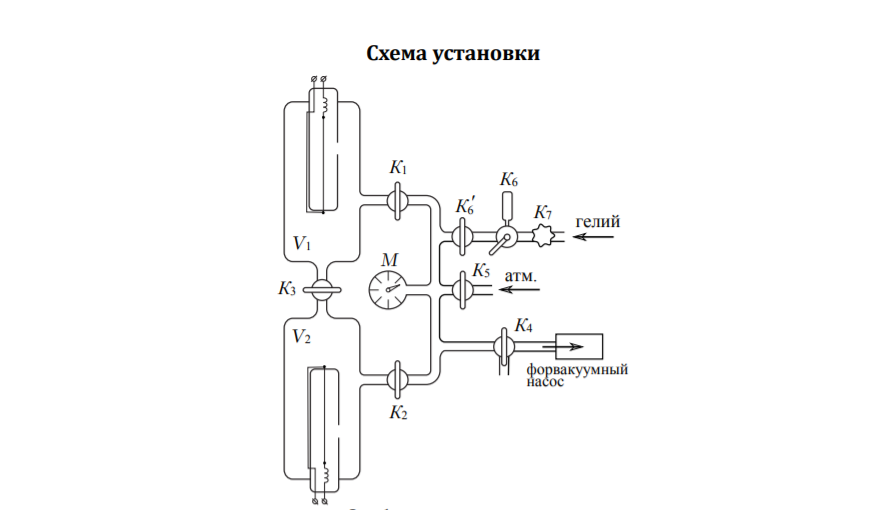
\includegraphics [scale=1]{ установка.png}}
	\caption{Экспериментальная установка}
\end{figure}

Особенности установки: Кран К4 изолирует форвакуумный насос от установки. Для подачи воздуха в установку служит кран К5.
Устройство и назначение кранов К6 и К7 подачи гелия соответствуют основному описанию. Дополнительный кран К'6 служит для вакуумной изоляции установки от системы подачи гелия. Краны К4, К5 и К'6 обладают повышенной вакуумплотностью и хорошо изолируют установку от протечек.


\newpage

\textbf{Результаты измерений и обработка данных:}
\begin{enumerate}
\item Начальные условия и погрешности:
$V = V_1 = V_2 = (775\pm 10) \text{см}^3$ - Объемы сосудов установки.


Инструментальная погрешность манометра - 0,5 кгс/см$^2$.

$L/S = (5,3 \pm 0,1)$1/см,  где L, S - длина и сечение трубки между двумя сосудами.

$P_{\text{атм}}$ = 738 мм.рт.ст. -- атмосферное давление 

\item Снимем зависимость напряжения на датчиках теплопроводности от времени при диффузии гелия и воздуха при различных давлениях в установке (40, 80, 120, 160, 200 Торр). Для сохранения результатов используется компьютерная программа, записывающая время и значение напряжения в отдельный файл.

\item По полученным данным строим графики зависимости ln U (t) для каждого давления.

	\begin{figure}[h]
	\center{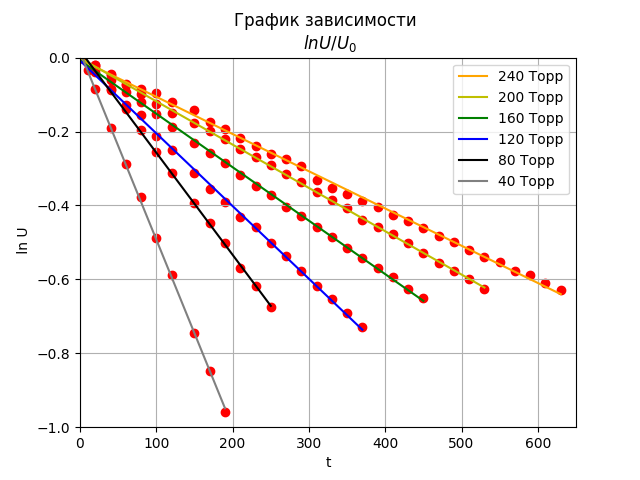
\includegraphics [scale=1]{ diffuzia.png}}
	\caption{}
\end{figure}

\item По коэффициентам наклона прямых можно определить коэффициенты диффузии по формуле: 
$$D = - \frac{1}{2} kV \frac{L}{S}, $$

$$ \sigma_D = D \sqrt{\big(\frac{\sigma_k}{k}\big)^2 + \big(\frac{\sigma_V }{V}\big)^2 + \big(\frac{\sigma_{L/S}}{L/S}\big)^2},$$ где $k$ - коэффициенты наклонов прямых

$$k = \frac{\left<\ln(U/U_0) t \right>}{\left<t^2 \right>},$$
$$\sigma_k = \frac{1}{\sqrt{n}}\sqrt{\frac{\left<\ln (U/U_0)^2\right>}{\left<t^2\right>}-k^2}.$$ 


	\begin{longtable}{|c|c|c|}
	\hline
	$P,$ торр & $D, \frac{\text{см}^2}{\text{c}}$ & $\sigma_D, \frac{\text{см}^2}{\text{c}}$\\
	 \hline
	40 & 10,4 & 0,1 \\ 
	\hline
	80 & 5,7 & 0,1 \\ 
	\hline
	120 &4,04& 0,09 \\ 
	\hline
	160& 2,97 & 0,08 \\ 
	\hline
	200& 2,41 & 0,07 \\ 
	\hline
	240& 2,07 & 0,07 \\ 
	\hline
	\caption{Давление и коэффициент диффузии}
\end{longtable}


\item Построим график зависимости D(1/P) и определим коэффициент диффузии при атмосферном давлении. Получим, что $D_{\text{атм}} = 1,01 \pm 0,04$ см$^2$/с (Табличное значение: $D_{\text{атм}}$ = 0,959 см$^2$/с )

	\begin{figure}[h]
	\center{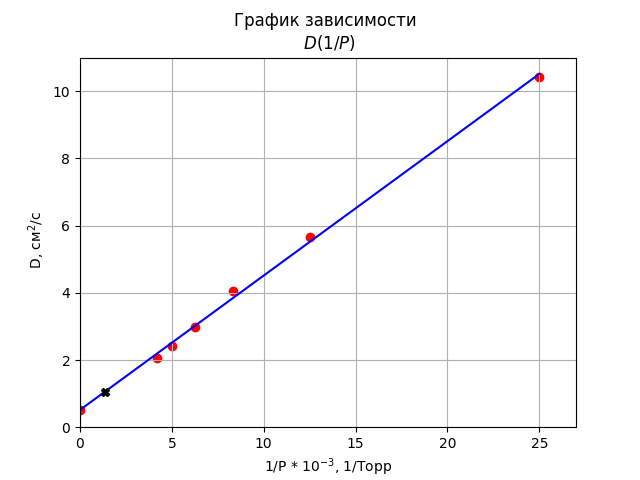
\includegraphics [scale=1]{ diffuzia_1.png}}
	\caption{}
\end{figure}

\newpage



\item Оценим по полученным результатам длину свободного пробега  атомов
гелия в воздухе $\lambda_{He}$ в условиях эксперимента, а также эффективное сечение столкновений атомов гелия с молекулами воздуха $\sigma$.   $$D = \frac{1}{3} \lambda_{He} \langle v \rangle,      
\langle v \rangle = \sqrt{\frac{8RT}{\pi \mu}}, \; \sigma = \frac{kT}{\sqrt{2}\lambda_{He} P},$$.

Получим, $\lambda_{He} = (208 \pm 6)\cdot 10^{-9}$ м, 

 $\sigma = (0,19 \pm 0,01)\cdot 10^{-18}$ м$^2$. 
 
 Табличные значения: $\lambda_{He} = 200\cdot 10^{-9}$ м.
 
 $\sigma = 0,2 \cdot 10^{-18}$ м$^2$.


\item Проверим утверждения о независимости коэффициента взаимной
диффузии от пропорций компонентов, проведем измерения коэффициента диффузии примеси воздуха в гелии (P$_He$ = 0,9 $P_0$, $P_{\text {возд.}}$ = 0,1 $P_0$, $P_0$ = 40 Торр). Можно заметить, что прямые не совпадают, это значит, что коэффициенты различны. Это связано с тем, что время измерения изменения напряжения в случае примеси воздуха в гелии мало, так же малость времени измерения можно понять по разбросу точек в этом случае.

	\begin{figure}[h]
	\center{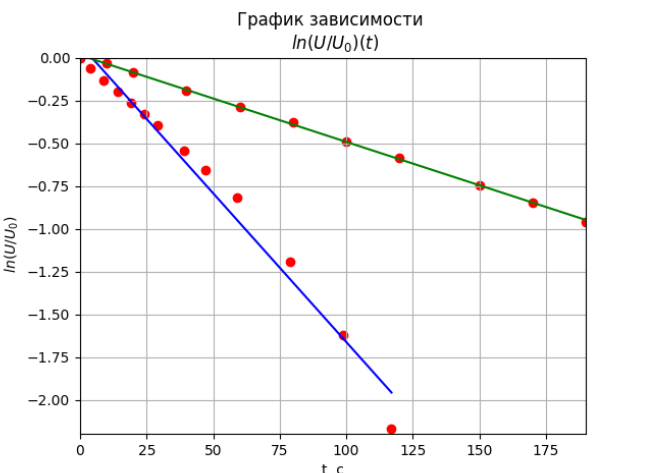
\includegraphics [scale=1]{ diff.png}}
	\caption{}
\end{figure}


\textbf{Обсуждение результатов:} В ходе данной работы мы регистрировали зависимости концентрации гелия в воздухе от времени с помощью датчиков теплопроводности при разных начальных давлениях смеси газов. Мы хотели подтвердить утверждения о независимости коэффициента взаимной диффузии от пропорций компонентов, однако при выполнении работы, мы получали низкое напряжение на датчиках теплоемкости и это не дало снять необходимое количество точек для того, чтобы величины можно было сравнивать. 


\textbf{Вывод:}
Мы определили коэффициент диффузии по результатам измерений  $D_{\text{атм}} = 1,01 \pm 0,04$ см$^2$/с что практически совпадает с табличным значением.
Также мы определили длину свободного пробега атомов гелия в воздухе  $\lambda_{He} = (208 \pm 6)\cdot 10^{-9}$ м и эффективное сечение столкновения атомов гелия с молекулами воздуха  
$\sigma = 0,2 \cdot 10^{-18}$ м$^2$. Полученные значения также практически совпадают с табличными.

\end{enumerate}
\end{document}